% Source: Zhou, physical PDF pp. 54--58 (printed pp. 38--42).
% Graphics: Figure 3.1 is transcribed as an editable native TikZ schematic of
% the two perpendicular cylinders and the source axes.

% ZHOU-SOURCE-PAGE: 54 PRINTED: 38
Since the $(\sec x+\tan x)$ term occurs in the derivative, we also have

\begin{equation*}
  \frac{d\ln\lvert\sec x+\tan x\rvert}{dx}
  =\frac{\sec x(\sec x+\tan x)}{(\sec x+\tan x)}
  =\sec x
\end{equation*}

\begin{equation*}
  \Rightarrow \int \sec x\,dx=\ln\lvert\sec x+\tan x\rvert+c
\end{equation*}

and

\begin{equation*}
  \int_{0}^{\pi/6}\sec x\,dx
  =\ln\bigl(\sec(\pi/6)+\tan(\pi/6)\bigr)
   -\ln\bigl(\sec(0)+\tan(0)\bigr)
  =\ln(\sqrt{3}).
\end{equation*}

\subsubsection*{Applications of integration}

\problem{A. Suppose that two cylinders each with radius 1 intersect at right angles and their centers also intersect. What is the volume of the intersection?}

\solution
This problem is an application of integration to volume calculation. For these applied
problems, the most difficult part is to correctly formulate the integration. The general
integration function to calculate 3D volume is

\begin{equation*}
  V=\int_{z_1}^{z_2}A(z)\,dz,
\end{equation*}

where $A(z)$ is the cross-sectional area of the solid cut by a plane perpendicular to the
$z$-axis at coordinate $z$. The key here is to find the right expression for cross-sectional
area $A$ as a function of $z$.

Figure 3.1 gives us a clue. If you cut the intersection by a horizontal plane, the cut will
be a square with side-length $\sqrt{(2r)^2-(2z)^2}$. Taking advantage of symmetry, we can
calculate the total volume as

\begin{equation*}
  2\times\int_{0}^{r}\left[(2r)^2-(2z)^2\right]dz
  =8\times\left[r^2z-\frac{z^3}{3}\right]_{0}^{r}
  =\frac{16}{3}r^3=\frac{16}{3}.
\end{equation*}

An alternative approach requires even better 3D imagination. Let's imagine a sphere that is
inscribed inside both cylinders, so it is inscribed inside the intersection as well. The sphere
should have a radius of $r/2$. At each cut perpendicular to the $z$-axis, the circle from the
sphere is inscribed in the square from the intersection as well. So
$A_{\mathrm{circle}}=\frac{\pi}{4}A_{\mathrm{square}}$. Since it's true for all $z$ values, we have

\begin{equation*}
  V_{\mathrm{sphere}}=\frac{4}{3}\pi\left(\frac{r}{2}\right)^3
  =\frac{\pi}{4}V_{\mathrm{intersection}}
  \Rightarrow V_{\mathrm{intersection}}=\frac{16}{3}r^3=\frac{16}{3}.
\end{equation*}

% ZHOU-SOURCE-PAGE: 55 PRINTED: 39
\begin{figure}[t]
  \centering
  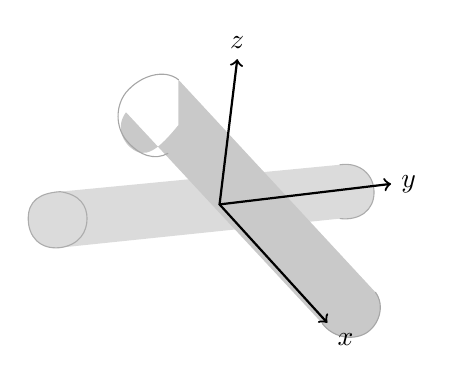
\begin{tikzpicture}[scale=0.9, line cap=round, line join=round]
    % Editable perspective schematic of the Steinmetz intersection shown in
    % the source.  The rear cylinder is aligned with the y-axis.
    \fill[gray!28] (-2.25,0.18) -- (1.70,0.56)
      .. controls (1.98,0.60) and (2.18,0.42) .. (2.18,0.17)
      .. controls (2.18,-0.08) and (1.98,-0.23) .. (1.70,-0.20)
      -- (-2.25,-0.61)
      .. controls (-2.54,-0.64) and (-2.70,-0.45) .. (-2.70,-0.20)
      .. controls (-2.70,0.05) and (-2.54,0.16) .. (-2.25,0.18);
    \draw[gray!65] (-2.25,0.18) .. controls (-2.54,0.16) and (-2.70,0.05) .. (-2.70,-0.20)
      .. controls (-2.70,-0.45) and (-2.54,-0.64) .. (-2.25,-0.61)
      .. controls (-1.97,-0.57) and (-1.87,-0.38) .. (-1.87,-0.20)
      .. controls (-1.87,-0.02) and (-1.97,0.14) .. (-2.25,0.18);
    \draw[gray!65] (1.70,0.56) .. controls (1.98,0.60) and (2.18,0.42) .. (2.18,0.17)
      .. controls (2.18,-0.08) and (1.98,-0.23) .. (1.70,-0.20);
    % The second cylinder runs along the diagonal x-axis.
    \fill[gray!42] (-0.58,1.76) -- (2.20,-1.24)
      .. controls (2.34,-1.43) and (2.25,-1.71) .. (2.06,-1.82)
      .. controls (1.86,-1.93) and (1.59,-1.87) .. (1.45,-1.68)
      -- (-1.32,1.30)
      .. controls (-1.47,1.10) and (-1.38,0.86) .. (-1.18,0.75)
      .. controls (-0.98,0.65) and (-0.78,0.88) .. (-0.58,1.12)
      -- cycle;
    \draw[gray!70] (-0.58,1.76) .. controls (-0.78,1.92) and (-1.12,1.82) .. (-1.32,1.58)
      .. controls (-1.47,1.39) and (-1.47,1.10) .. (-1.32,0.91)
      .. controls (-1.13,0.68) and (-0.91,0.62) .. (-0.73,0.72);
    \draw[gray!70] (2.20,-1.24) .. controls (2.34,-1.43) and (2.25,-1.71) .. (2.06,-1.82)
      .. controls (1.86,-1.93) and (1.59,-1.87) .. (1.45,-1.68);
    % Coordinate axes at the common centre, as in the source graphic.
    \draw[->,thick] (0,0) -- (2.42,0.29) node[right] {$y$};
    \draw[->,thick] (0,0) -- (1.52,-1.67) node[below right] {$x$};
    \draw[->,thick] (0,0) -- (0.25,2.05) node[above] {$z$};
  \end{tikzpicture}
  \caption{Interaction of two cylinders}
  \label{fig:zhou-figure-3-1}
\end{figure}

\problem{B. The snow began to fall some time before noon at a constant rate. The city of Cambridge sent out a snow plow at noon to clear Massachusetts Avenue from MIT to Harvard. The plow removed snow at a constant volume per minute. At 1 pm, it had moved 2 miles and at 2 pm, 3 miles. When did the snow begin to fall?}

\solution
Let's denote noon as time 0 and assume snow began to fall $T$ hours before noon. The speed
at which the plow moves is inversely related to the vertical cross-sectional area of the snow:
$v=c_1/A(t)$, where $v$ is the speed of the plow, $c_1$ is a constant representing the volume
of snow that the plow can remove every hour and $A(t)$ is the cross-sectional area of the snow.
If $t$ is defined as the time after noon, we also have $A(t)=c_2(t+T)$, where $c_2$ is the rate
of cross-sectional area increase per hour (since the snow falls at a constant rate). So

\begin{equation*}
  v=\frac{c_1}{c_2(t+T)}=\frac{c}{t+T}
\end{equation*}

where $c=\frac{c_1}{c_2}$. Taking the integration, we have

\begin{equation*}
  \int_{0}^{1}\frac{c}{T+t}\,dt
  =c\ln(1+T)-c\ln T
  =c\ln\left(\frac{1+T}{T}\right)=2,
\end{equation*}

\begin{equation*}
  \int_{0}^{2}\frac{c}{T+t}\,dt
  =c\ln(2+T)-c\ln T
  =c\ln\left(\frac{2+T}{T}\right)=3.
\end{equation*}

From these two equations, we get

\begin{equation*}
  \left(\frac{1+T}{T}\right)^3
  =\left(\frac{2+T}{T}\right)^2
  % ZHOU-SOURCE-ERROR: The printed source has T^2-T+1=0, although the
  % following root solves T^2+T-1=0. The visible source equation is retained.
  \Rightarrow T^2-T+1=0
  \Rightarrow T=\frac{\sqrt{5}-1}{2}.
\end{equation*}

% ZHOU-SOURCE-PAGE: 56 PRINTED: 40
Overall, this question, although fairly straightforward, tests analytical skills,
integration knowledge and algebra knowledge.

\subsubsection*{Expected value using integration}

Integration is used extensively to calculate the unconditional or conditional expected value
of continuous random variables. In Chapter 4, we will demonstrate its value in probability and
statistics. Here we just use one example to show its application:

\problem{If $X$ is a standard normal random variable, $X\sim N(0,1)$, what is $E[\lvert X\rvert\mid X>0]$?}

\solution
Since $X\sim N(0,1)$, the probability density function of $x$ is

\begin{equation*}
  f(x)=\frac{1}{\sqrt{2\pi}}e^{-x^2/2}
\end{equation*}

and we have

\begin{equation*}
  E[\lvert X\rvert\mid X>0]
  =\int_{0}^{\infty}xf(x)\,dx
  =\int_{0}^{\infty}\frac{x}{\sqrt{2\pi}}e^{-x^2/2}\,dx.
\end{equation*}

Because $d(-1/2x^2)=-x$ and $\int e^u\,dy=e^u+c$, where $c$ is an arbitrary constant,
it is obvious that we can use integration by substitution by letting $u=-1/2x^2$. Replace
$e^{-1/2x^2}$ with $e^u$ and $x\,dx$ with $-du$, we have

\begin{equation*}
\begin{aligned}
  \int_{0}^{\infty}x\frac{1}{\sqrt{2\pi}}e^{-x^2/2}\,dx
  &=\int_{0}^{-\infty}-\frac{1}{\sqrt{2\pi}}e^u\,du
   =-\frac{1}{\sqrt{2\pi}}\left[e^u\right]_{0}^{-\infty} \\
  &=-\frac{1}{\sqrt{2\pi}}(0-1)=\frac{1}{\sqrt{2\pi}},
\end{aligned}
\end{equation*}

where $[e^u]_{0}^{-\infty}$ is determined by $x=0\Rightarrow u=0$ and
$x=\infty\Rightarrow u=-\infty$.

\begin{equation*}
  \therefore\quad E[\lvert X\rvert\mid X>0]=\frac{1}{\sqrt{2\pi}}.
\end{equation*}

\subsection{Partial Derivatives and Multiple Integrals}

\textbf{Partial derivative:} $w=f(x,y)\Rightarrow$

\begin{equation*}
  \frac{\partial w}{\partial x}(x_0,y_0)
  =\lim_{\Delta x\to0}\frac{f(x_0+\Delta x,y_0)-f(x_0,y_0)}{\Delta x}
  =f_x.
\end{equation*}

\textbf{Second order partial derivatives:}

\begin{equation*}
  \frac{\partial^2f}{\partial x^2}=\frac{\partial}{\partial x}\left(\frac{\partial f}{\partial x}\right),
  \qquad
  \frac{\partial^2f}{\partial x\partial y}
  =\frac{\partial}{\partial x}\left(\frac{\partial f}{\partial y}\right)
  =\frac{\partial}{\partial y}\left(\frac{\partial f}{\partial x}\right).
\end{equation*}

\textbf{The general chain rule:} Suppose that $w=f(x_1,x_2,\ldots,x_m)$ and that each of
variables $x_1,x_2,\ldots,x_n$ is a function of the variables $t_1,t_2,\ldots,t_n$. If all these
functions have continuous first-order partial derivatives, then

\begin{equation*}
  \frac{\partial w}{\partial t_i}
  =\frac{\partial w}{\partial x_1}\frac{\partial x_1}{\partial t_i}
   +\frac{\partial w}{\partial x_2}\frac{\partial x_2}{\partial t_i}
   +\cdots+
   \frac{\partial w}{\partial x_m}\frac{\partial x_m}{\partial t_i}
\end{equation*}

for each $i$, $1\leq i\leq n$.

% ZHOU-SOURCE-PAGE: 57 PRINTED: 41
\textbf{Changing Cartesian integrals into polar integrals:} The variables in two-dimension
plane can be mapped into polar coordinates: $x=r\cos\theta$, $y=r\sin\theta$. The integration
in a continuous polar region $R$ is converted to

\begin{equation*}
  \iint_R f(x,y)\,dx\,dy
  =\iint_R f(r\cos\theta,r\sin\theta)\,r\,dr\,d\theta.
\end{equation*}

\problem{Calculate $\displaystyle\int_{0}^{\infty}e^{-x^2/2}\,dx$.}

\solution
Hopefully you happen to remember that the probability density function (pdf) of the standard
normal distribution is $f(x)=\frac{1}{\sqrt{2\pi}}e^{-x^2/2}$. By definition, we have

\begin{equation*}
  \int_{-\infty}^{\infty}f(x)\,dx
  =\int_{-\infty}^{\infty}\frac{1}{\sqrt{2\pi}}e^{-x^2/2}\,dx
  =2\int_{0}^{\infty}\frac{1}{\sqrt{2\pi}}e^{-x^2/2}\,dx
  =1
  \Rightarrow \int_{0}^{\infty}e^{-x^2/2}\,dx=\sqrt{\frac{\pi}{2}}.
\end{equation*}

If you've forgotten the pdf of the standard normal distribution or if you are specifically asked
to prove

\begin{equation*}
  \int_{-\infty}^{\infty}\frac{1}{\sqrt{2\pi}}e^{-x^2/2}\,dx=1,
\end{equation*}

you will need to use polar integrals to solve the problem:

\begin{equation*}
\begin{aligned}
  &\int_{-\infty}^{\infty}e^{-x^2/2}\,dx
   \int_{-\infty}^{\infty}e^{-y^2/2}\,dy \\
  &\quad=\int_{-\infty}^{\infty}\int_{-\infty}^{\infty}
   e^{-(x^2+y^2)/2}\,dx\,dy \\
  &\quad=\int_{0}^{2\pi}\int_{0}^{\infty}
   e^{-(r^2\cos^2\theta+r^2\sin^2\theta)/2}\,r\,dr\,d\theta \\
  &\quad=\int_{0}^{\infty}\int_{0}^{2\pi}e^{-r^2/2}r\,d\theta\,dr \\
  &\quad=-\int_{0}^{\infty}e^{-r^2/2}\,d(-r^2/2)\int_{0}^{2\pi}d\theta \\
  &\quad=-\left[e^{-r^2/2}\right]_{0}^{\infty}\left[\theta\right]_{0}^{2\pi}=2\pi.
\end{aligned}
\end{equation*}

Since $\int_{-\infty}^{\infty}e^{-x^2/2}\,dx=\int_{-\infty}^{\infty}e^{-y^2/2}\,dy$, we have

\begin{equation*}
  \int_{-\infty}^{\infty}e^{-x^2/2}\,dx=\sqrt{2\pi}
  \Rightarrow \int_{0}^{\infty}e^{-x^2/2}\,dx=\sqrt{\frac{\pi}{2}}.
\end{equation*}

\subsection{Important Calculus Methods}

\subsubsection*{Taylor's series}

One-dimensional Taylor's series expands function $f(x)$ as the sum of a series using the
derivatives at a point $x=x_0$:

\begin{equation*}
  f(x)=f(x_0)+f'(x_0)(x-x_0)+\frac{f''(x_0)}{2!}(x-x_0)^2
  +\cdots+\frac{f^{(n)}(x_0)}{n!}(x-x_0)^n+\cdots.
\end{equation*}

% ZHOU-SOURCE-PAGE: 58 PRINTED: 42
If $x_0=0$,

\begin{equation*}
  f(x)=f(0)+f'(0)x+\frac{f''(0)}{2!}x^2+\cdots+\frac{f^{(n)}(0)}{n!}x^n+\cdots.
\end{equation*}

Taylor's series are often used to represent functions in power series terms. For example,
Taylor's series for three common transcendental functions, $e^x$, $\sin x$ and $\cos x$, at
$x_0=0$ are

\begin{equation*}
  e^x=\sum_{n=0}^{\infty}\frac{x^n}{n!}
  =1+\frac{x}{1!}+\frac{x^2}{2!}+\frac{x^3}{3!}+\cdots,
\end{equation*}

\begin{equation*}
  \sin x=\sum_{n=0}^{\infty}\frac{(-1)^n x^{2n+1}}{(2n+1)!}
  =x-\frac{x^3}{3!}+\frac{x^5}{5!}-\frac{x^7}{7!}+\cdots,
\end{equation*}

\begin{equation*}
  \cos x=\sum_{n=0}^{\infty}\frac{(-1)^n x^{2n}}{(2n)!}
  =1-\frac{x^2}{2!}+\frac{x^4}{4!}-\frac{x^6}{6!}+\cdots.
\end{equation*}

The Taylor's series can also be expressed as the sum of the $n$th-degree Taylor polynomial
$T_n(x)=f(x_0)+f'(x_0)(x-x_0)+\frac{f''(x_0)}{2!}(x-x_0)^2+\cdots+
\frac{f^{(n)}(x_0)}{n!}(x-x_0)^n$ and a remainder $R_n(x)$:

\begin{equation*}
  f(x)=T_n(x)+R_n(x).
\end{equation*}

For some $\tilde{x}$ between $x_0$ and $x$,

\begin{equation*}
  R_n(x)=\frac{f^{(n+1)}(\tilde{x})}{(n+1)!}\lvert x-x_0\rvert^{n+1}.
\end{equation*}

Let $M$ be the maximum of $\lvert f^{(n+1)}(\tilde{x})\rvert$ for all $\tilde{x}$ between
$x_0$ and $x$, we get constraint

\begin{equation*}
  \lvert R_n(x)\rvert\leq\frac{M\times\lvert x-x_0\rvert^{n+1}}{(n+1)!}.
\end{equation*}

\problem{A. What is $i^i$?}

\solution
The solution to this problem uses Euler's formula, $e^{i\theta}=\cos\theta+i\sin\theta$,
which can be proven using Taylor's series. Let's look at the proof. Applying Taylor's series to
$e^{i\theta}$, $\cos\theta$ and $\sin\theta$, we have

\begin{equation*}
  e^{i\theta}=1+\frac{i\theta}{1!}+\frac{(i\theta)^2}{2!}+\frac{(i\theta)^3}{3!}
  +\frac{(i\theta)^4}{4!}+\cdots
  =1+\frac{i\theta}{1!}-\frac{\theta^2}{2!}-\frac{i\theta^3}{3!}
  +\frac{\theta^4}{4!}+\frac{i\theta^5}{5!}+\cdots,
\end{equation*}

\begin{equation*}
  \cos\theta=1-\frac{\theta^2}{2!}+\frac{\theta^4}{4!}-\frac{\theta^6}{6!}+\cdots,
\end{equation*}

\begin{equation*}
  \sin\theta=\theta-\frac{\theta^3}{3!}+\frac{\theta^5}{5!}-\frac{\theta^7}{7!}+\cdots
  \Rightarrow i\sin\theta=\frac{i\theta}{1!}-\frac{i\theta^3}{3!}
  +\frac{i\theta^5}{5!}-\frac{i\theta^7}{7!}+\cdots.
\end{equation*}
